
\documentclass{article}
\usepackage{CJK}
\usepackage{graphicx}
\usepackage[includemp,body={398pt,550pt},footskip=30pt,%
            marginparwidth=60pt,marginparsep=10pt]{geometry}
\usepackage{graphicx}
\usepackage{subfigure}

 \begin{CJK*}{GBK}{song}
  \renewcommand\figurename{图}
\begin{document}
\begin{figure}
\begin{minipage}[t]{0.5\textwidth}
\centering
\includegraphics[width=2.2in]{pic1.eps}
\caption{fig1}
\label{fig:side:a}
\end{minipage}%
\begin{minipage}[t]{0.5\textwidth}
\centering
\includegraphics[width=2.2in]{pic.eps}
\caption{fig2}
\label{fig:side:b}
\end{minipage}
\end{figure}
\begin{figure}
  \centering
  \subfigure[Small Box with a Long Caption]{
    \label{fig:subfig:a} %% label for first subfigure
    \includegraphics[width=1.0in]{pic1.eps}}
  \hspace{1in}
  \subfigure[Big Box]{
    \label{fig:subfig:b} %% label for second subfigure
    \includegraphics[width=1.5in]{pic.eps}}
  \caption{Two Subfigures}
  \label{fig:subfig} %% label for entire figure
\end{figure}

 \paragraph{}
\clearpage
\end{CJK*}
\end{document}

% \documentclass[10pt, a4paper, parskip=full]{article}
% % twoside can be added if two sided margin layout is desired
% \usepackage[a4paper,vmargin={30mm, 20mm},hmargin={30mm, 25mm},includeheadfoot]{geometry}
% \usepackage{amsmath}
% \usepackage[UTF8]{ctex}
% \usepackage{xpinyin}
% \xpinyinsetup{ratio=0.5, vsep=1em, multiple={\color{red}}, font=Liberation Sans}
% \usepackage{fontspec,xunicode}
% \setCJKmainfont[]{WenQuanYi Micro Hei}
% \defaultfontfeatures{Mapping=tex-text, Scale=MatchLowercase}
% % what does this do? -- influences how quotes are rendered
% \setmainfont[Scale=1]{Open Sans}
% \setmonofont{Liberation Mono}
% \DeclareMathSizes{10}{10}{8}{7}
% \usepackage[english, ngerman]{babel}
% \selectlanguage{ngerman}
% \begin{document}
% There is latin text here.
% \begin{pinyinscope} 我有一个送给你的礼物.\end{pinyinscope}
% \end{document}

%%% 
\documentclass{book}
\usepackage{CJKutf8}
\begin{document}
\begin{CJK*}{UTF8}{gbsn}

  \chapter{某章}
  内容……

  \chapter{某章}
  内容……

  \clearpage\end{CJK*}
\end{document}

%%% 
% Compile with xelatex
% UTF-8 encoding
\documentclass{article}
\usepackage{xeCJK}
\setCJKmainfont{SimSun}
\begin{document}
文章内容
\end{document}

%%%
\documentclass{article}
\usepackage{CJKutf8}

\begin{document}

\begin{CJK*}{UTF8}{gbsn}  %UTF8 is the encoding and gbsn is the font to be used. You can use gbsn or gkai fonts for simplified characters, and bmsi or bkai for traditional characters. 

  \section{前言}
  在该第一部分中的一些额外的元素可以被添加。巴贝尔包将采取的翻译服务.

  \section{关于数学部分}
  在本节中的一些数学会使用数学模型含中文字符显示。

\end{CJK*}

\vspace{0.5cm} % A white space

\noindent
You can also insert Latin text in your document

\vspace{0.5cm}

\noindent
\begin{CJK*}{UTF8}{bsmi}
  這是一個傳統的中國文字
\end{CJK*}

\end{document}

%%% 
\documentclass{article}

\usepackage{xeCJK}

\setCJKmainfont{simsun.ttf}
\setCJKsansfont{simhei.ttf}
\setCJKmonofont{simfang.ttf}

\begin{document}

\section{前言}
在该第一部分中的一些额外的元素可以被添加。巴贝尔包将采取的翻译服务.

\section{关于数学部分}
在本节中的一些数学会使用数学模型含中文字符显示。

\vspace{0.5cm}

這是一個傳統的中國文字
\end{document}

%%% 
\documentclass{ctexart}

\setCJKmainfont{SimSun.ttf}
\setCJKsansfont{SimHei.ttf}
\setCJKmonofont{SimFang.ttf}

\begin{document}

\tableofcontents

\begin{abstract}
  这是在文件的开头的介绍文字.本文的主要话题的简短说明.
\end{abstract}

\section{ 前言 }
在该第一部分中的一些额外的元素可以被添加。巴贝尔包将采取的翻译服务.

\section{关于数学部分}
在本节中的一些数学会使用数学模型含中文字符显示。

這是一個傳統的中國文字

\end{document}

%%%
\DeclareSymbolFontAlphabet{\mathrm}    {operators}  
 \DeclareSymbolFontAlphabet{\mathnormal}{letters}  
 \DeclareSymbolFontAlphabet{\mathcal}   {symbols}  
 \DeclareMathAlphabet      {\mathbf}{OT1}{cmr}{bx}{n}  
 \DeclareMathAlphabet      {\mathsf}{OT1}{cmss}{m}{n}  
 \DeclareMathAlphabet      {\mathit}{OT1}{cmr}{m}{it}  
 \DeclareMathAlphabet      {\mathtt}{OT1}{cmtt}{m}{n}  
   
 This must be completed by the previous declarations  
   
 \DeclareSymbolFont{operators}   {OT1}{cmr} {m}{n}  
 \DeclareSymbolFont{letters}     {OML}{cmm} {m}{it}  
 \DeclareSymbolFont{symbols}     {OMS}{cmsy}{m}{n}  
     
 so that we know precisely to which font correspond each  
 math command:  
   
 1 \mathrm is the normal upright Roman font   
     
 2 \mathnormal is the normal math italic font:  
  $\mathnormal{a}$ and $a$ give the same result  
     
 3 \mathcal is the special calligraphic font for uppercase  
  letters only  
   
 4 \mathbf gives upright Roman boldface letters  
   
 5 \mathsf gives upright sans serif letters  
   
 6 \mathit gives text italic letters: $different\ne\mathit  
  {different}$  
   
 7 \mathtt gives upright letters from the typewriter type  
  font


在latex中,对于双栏格式的排版,

插入一栏图片时,使用的是\begin{figure}……\end{figure} ,

插入双栏图片时需在figure的上标中加入符号“*”,如\begin{figure*}……\end{figure*}。
1.在latex插入一张图片(占一栏)比较简单,插入一张图片的代码如下:
\begin{figure}{!h} *h插在引用处,t插在本段文本所在栏的顶部,b插在本段文本所在栏的底部,p单独占一页。
\centering %使插入的图片居中显示
\includegraphics[height=5cm ,width=8cm,angle=0,scale=]{fig.eps}
\caption{Example twig query and documents } %插入图片的标题,一般放在图片的下方,放在表格的上方
\end{figure}
关键性的语句是:\includegraphics[选项]{图片.eps}
选项:height %指定图片的高度
width %指定图片的宽度
angle %指定图片旋转的角度
还有一个指标叫scale,之缩放图形。

2.在latex插入多张图片(占双栏)就不是那么简单了,笔者知道有两种方法:
法一:使用\begin{minipage}[pos]{width} text \end{minipage} 

\begin{figure*}
\centering
\begin{minipage}[!htbp]{0.3\linewidth}
\includegraphics[width=1.5in,angle=-90]{52.eps}
%\caption{fig1}
\label{fig:side:a}
\end{minipage}%
\begin{minipage}[!htbp]{0.3\linewidth}
\includegraphics[width=1.5in,angle=-90]{51.eps}
%\caption{fig2}
\label{fig:side:b}
\end{minipage}
\begin{minipage}[!htbp]{0.3\linewidth}
\includegraphics[width=1.5in,angle=-90]{53.eps}
%\caption{fig3}
\label{fig:side:c}
\end{minipage}
\caption{3 figure}
\end{figure*}
注:笔者不太喜欢这种方法,原因是这种插入方式如果在每个图中使用\caption{fig3 name}给图片做注释的时候不是把三个图片当做一个figure,而是每个图片即每个minipage各使用一个fig标记,三个mingpage相当于三个图片了,当然也可以不单独对每个图片写个\caption,而是在\caption{3figure}中对每个figure进行解释说明,所以笔者推崇第二种方法。当然,笔者也许不知道如何设置,有望业内人士指教。

法二:使用subfigure命令,但必须在导演区加入\usepackage{subfigure},否则无法编译过去。

\begin{figure*}[!t]
\centering
\subfigure[Number of elements read] {\includegraphics[height=2in,width=2in,angle=-90]{52.eps}}
\subfigure[Size of disk files scanned] {\includegraphics
[height=2in,width=2in,angle=-90]{51.eps}}
\subfigure[Execution time] {\includegraphics[height=2in,width=2in,angle=-90]{53.eps}}
\caption{ PathStack versus TJFast using XMark data }
\label{fig5}
\end{figure*}

这种方法很好,即插入三个子图,可以将三个图片合成一个大图,而且每个图片还可以添加caption,即于subfigure[*]中*内进行解释说明。

\begin{minipage}[b][12cm][t]{1.00\textwidth}
%\centering
Test LaTex
\begin{align*}
1&.aaa\\
2&.bbb\\
3&.ccc
\end{align*}
\end{minipage}

\begin{minipage}{0.2\textwidth}
\begin{tabular}{|c|c|c|}
\hline
 A & B & C \\
\hline
 1 & 2 & 3  \\
\hline 
 4 & 5 & 6 \\
\hline
\end{tabular}
\end{minipage}

\begin{figure*}
\centering
\subfigure[Input]{
\begin{minipage}[b]{0.23\linewidth}
\includegraphics[width=1\linewidth]{a1.jpg}\vspace{4pt}
\includegraphics[width=1\linewidth]{a2.jpg}\vspace{4pt}
\includegraphics[width=1\linewidth]{a3.jpg}\vspace{4pt}
\includegraphics[width=1\linewidth]{a4.jpg}
\end{minipage}}
\subfigure[CE]{
\begin{minipage}[b]{0.23\linewidth}
\includegraphics[width=1\linewidth]{b1.jpg}\vspace{4pt}
\includegraphics[width=1\linewidth]{b2.jpg}\vspace{4pt}
\includegraphics[width=1\linewidth]{b3.jpg}\vspace{4pt}
\includegraphics[width=1\linewidth]{b4.jpg}
\end{minipage}}
\subfigure[Ours]{
\begin{minipage}[b]{0.23\linewidth}
\includegraphics[width=1\linewidth]{c1.jpg}\vspace{4pt}
\includegraphics[width=1\linewidth]{c2.jpg}\vspace{4pt}
\includegraphics[width=1\linewidth]{c3.jpg}\vspace{4pt}
\includegraphics[width=1\linewidth]{c4.jpg}
\end{minipage}}
\subfigure[GT]{
\begin{minipage}[b]{0.23\linewidth}
\includegraphics[width=1\linewidth]{d1.jpg}\vspace{4pt}
\includegraphics[width=1\linewidth]{d2.jpg}\vspace{4pt}
\includegraphics[width=1\linewidth]{d3.jpg}\vspace{4pt}
\includegraphics[width=1\linewidth]{d4.jpg}
\end{minipage}}
\caption{description of figure}
\end{figure*}

说明: 
1)subfigure本身不支持内部图片换行,所以结合minipage使用 
2)minipage可以在每一个includegraphics后跟双斜杠“\”表示换行,也可以像上面代码中写的使用”\vspace{4.pt}”来控制垂直间距,但是需要注意的是”\vspace{4.pt}”必须紧跟在对应的includegraphics,不然得不到想要的结果。 
3)使用figure和subfigure必须引相应的包”\usepackage{graphicx}”和”\usepackage{subfigure}”

\begin{figure}   
   \centering   
   \begin{minipage}[b]{.33\textwidth}   
     \centering   
     \includegraphics[width=2cm]{graphic.eps}   
   \end{minipage}%   
   \begin{minipage}[b]{.33\textwidth}   
     \centering   
     \includegraphics[width=2cm,angle=-30]{graphic.eps}   
   \end{minipage}\\[-10pt]   
   \begin{minipage}[t]{.33\textwidth}   
     \caption{Box with a Long Caption}   
   \end{minipage}%   
   \begin{minipage}[t]{.33\textwidth}   
     \caption{Rotated Box}   
   \end{minipage}%   
 \end{figure}  
 生成的图 27.7 和 27.8 中,图形的基 线和标题的第一行分别对齐。
  \includegraphics[width=2cm]{graphic.eps}    
  在这个例子中,需要注意:
  
 * 在最后一幅图后面用 \\ 来断行, \\ 的参数项 [-10pt] 使得图形与标题之间的距离比当前行距减少 10pt。这样做是让图形和标题更接近些,用户也可 自己选用合适的值。   
 * 包含图形的小页使用 [b] 选项,使得它们的参考点为 其最后一行的基线  
 * 包含标题小页使用 [t] 选项,使得它们的参考点为 其第一行的基线。   
 * 任何一个 \label 命令都必须和它相应的 \caption 命令在同一个小页中。
\setlength{\mathindent}{0pt}

\documentclass[margin=10pt]{standalone} 
\usepackage{tikz} 
%\input{mypgfmacrolibrary}
\usetikzlibrary{intersections} 
\begin{document} 
\begin{tikzpicture} 
\coordinate (O) at (0,0); 
\coordinate (A) at (2.0,2.0); 
\draw [name path = c1, red, thick] (A) circle [radius = 4cm]; 
\draw [name path = c2, green, thin] (A) ellipse (5.0cm and 2.0cm); 
\draw [execute at begin node={\global\let\t=\t},
       name intersections = {of = c1 and c2,total=\t}] 
(intersection-1) -- (intersection-2) -- (intersection-3) 
-- (intersection-4) -- cycle; 
\pgfmathsetmacro{\nr}{0}
\foreach \point in {1,...,\t}
  \filldraw[red] (intersection-\point) circle (0.5cm);
\end{tikzpicture} 
\end{document}

\documentclass[margin=10pt]{standalone}
\usepackage{tikz}
\usetikzlibrary{math}
\usepackage{ifthen}
\newcounter{count}
\begin{document}
\begin{tikzpicture} 
  \def\clr{red}% initial color
  \setcounter{count}{0}% initial counter 
  \foreach \col in {1,...,6}
  {
    \foreach \row in {1,...,3}
       {
         \stepcounter{count}
         \ifthenelse{\value{count}>6}{\def\clr{blue}}{}
         \draw[fill=\clr] (\col,\row) ellipse (1cm and 1cm);
       }
  }
\end{tikzpicture}
\end{document}

    \documentclass{article} 
    \usepackage{tikz} 
    \usetikzlibrary{calc,fadings,decorations.pathreplacing} 
    \usepackage[active,tightpage]{preview}
    \PreviewEnvironment{tikzpicture}
    \setlength\PreviewBorder{5pt}
    \pagestyle{empty} 
     
    %% helper macros
    \newcommand\pgfmathsinandcos[3]{% 
       \pgfmathsetmacro#1{sin(#3)}% 
       \pgfmathsetmacro#2{cos(#3)}% 
    } 
    \newcommand\LongitudePlane[3][current plane]{%
       \pgfmathsinandcos\sinEl\cosEl{#2} % elevation
       \pgfmathsinandcos\sint\cost{#3} % azimuth
       \tikzset{#1/.style={cm={\cost,\sint*\sinEl,0,\cosEl,(0,0)}}}
    }
    \newcommand\LatitudePlane[3][current plane]{%
       \pgfmathsinandcos\sinEl\cosEl{#2} % elevation
       \pgfmathsinandcos\sint\cost{#3} % latitude
       \pgfmathsetmacro\yshift{\cosEl*\sint}
       \tikzset{#1/.style={cm={\cost,0,0,\cost*\sinEl,(0,\yshift)}}} % 
    }
    \newcommand\DrawLongitudeCircle[2][1]{
       \LongitudePlane{\angEl}{#2}
       \tikzset{current plane/.prefix style={scale=#1}}
        % angle of "visibility" 
       \pgfmathsetmacro\angVis{atan(sin(#2)*cos(\angEl)/sin(\angEl))} %
       \draw[current plane] (\angVis:1) arc (\angVis:\angVis+180:1); 
       \draw[current plane,dashed] (\angVis-180:1) arc (\angVis-180:\angVis:1); 
    }
    \newcommand\DrawLatitudeCircle[2][1]{
       \LatitudePlane{\angEl}{#2}
       \tikzset{current plane/.prefix style={scale=#1}}
       \pgfmathsetmacro\sinVis{sin(#2)/cos(#2)*sin(\angEl)/cos(\angEl)} 
       % angle of "visibility"
       \pgfmathsetmacro\angVis{asin(min(1,max(\sinVis,-1)))}  
       \draw[current plane] (\angVis:1) arc (\angVis:-\angVis-180:1); 
       \draw[current plane,dashed] (180-\angVis:1) arc (180-\angVis:\angVis:1);
    }
     
    %% document-wide tikz options and styles
    \tikzset{%
       >=latex, % option for nice arrows 
       inner sep=0pt,%
       outer sep=2pt,%
       mark coordinate/.style={inner sep=0pt,outer sep=0pt,minimum size=3pt,fill=black,circle}%
    }
     
    \begin{document} 
     
    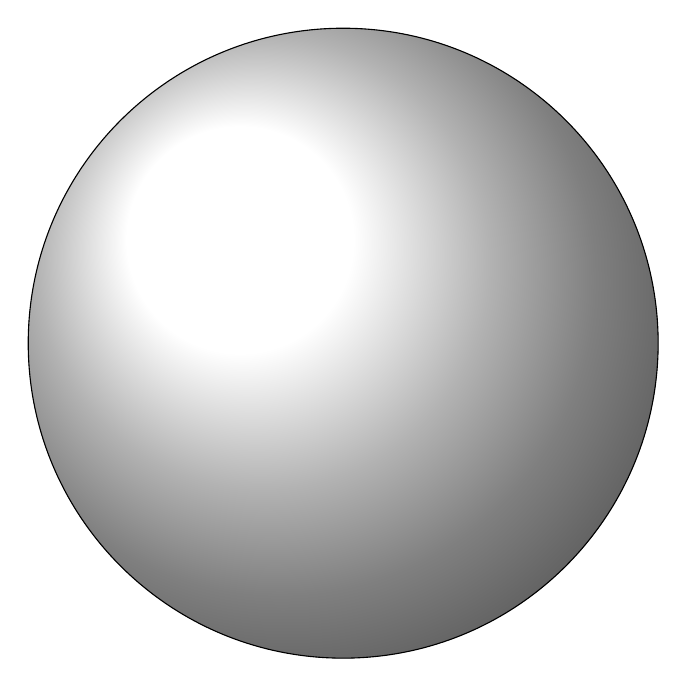
\begin{tikzpicture} % CENT
     
    %% some definitions 
    \def\R{4} % sphere radius
    \def\angEl{35} % elevation angle 
    \def\angAz{-105} % azimuth angle 
    \def\angPhi{-40} % longitude of point P 
    \def\angBeta{25} % latitude of point P 
     
    %% working planes
    \pgfmathsetmacro\H{\R*cos(\angEl)} % distance to north pole
    \tikzset{xyplane/.style={cm={cos(\angAz),sin(\angAz)*sin(\angEl),-sin(\angAz),cos(\angAz)*sin(\angEl),(0,-\H)}}}
    \LongitudePlane[xzplane]{\angEl}{\angAz}
    \LongitudePlane[pzplane]{\angEl}{\angPhi}
    \LongitudePlane[yzplane]{\angEl}{\angAz+90}
    \LatitudePlane[equator]{\angEl}{0}
     
    %% draw xyplane and sphere
    \fill[ball color=white] (0,0) circle (\R); % 3D lighting effect
    \draw (0,0) circle (\R);
     
    %% draw meridians and latitude circles
    \DrawLatitudeCircle[\R]{0} % equator
    %\DrawLatitudeCircle[\R]{\angBeta}
    \DrawLongitudeCircle[\R]{\angAz} % xzplane
    \DrawLongitudeCircle[\R]{\angAz+90} % yzplane
    \DrawLongitudeCircle[\R]{\angPhi} % pzplane
     
    \end{tikzpicture} 
    \end{document} 


